\subsection{Wizualizacja}
W celu zapewnienia użytkownikowi końcowemu zintegrowanego i spójnego środowiska wizualizacji całego procesu – od wgrania plików wejściowych po interakcję z modelem – zaprojektowano od podstaw interfejs oraz system renderowania.

Założeniem projektu była implementacja intuicyjnego, dynamicznego i responsywnego \textbf{interfejsu}[\ref{fig:rendering}] przy pomocy biblioteki \textit{PyQt} oraz języka \textit{QML}. Interfejs został zintegrowany z wydajnym systemem \textbf{renderingu}[\ref{fig:rendering}] GPU, wykorzystującym technologie \textit{OpenGL}, \textit{OpenCL} oraz język \textit{C}. Dodatkowo, użytkownik ma możliwość alternatywnego renderowania z wykorzystaniem biblioteki \textit{VisPy}.

Projekt rozwiązuje problem fragmentaryczności funkcji dostępnych w innych aplikacjach, oferując spójne środowisko do obsługi modeli 3D, obejmujące procesy tworzenia, modyfikacji, segmentacji oraz wizualizacji danych.

\vspace{10pt}
{\setlength{\parindent}{0pt}
\textbf{Rendering}
}

Rendering wykorzystuje plik .ply jako dane wejściowe do wczytania splatów. Splaty te są reprezentowane przez sześciany z dodatkowymi parametrami przechowywanymi w Shader Storage Buffer Object (SSBO), co umożliwia efektywny odczyt dużych ilości danych. Takie podejście jest szczególnie przydatne w przypadku scen zawierających nawet do dwóch milionów obiektów.

Do przechowywanych parametrów należą: \begin{itemize} \item pozycja, \item skala, \item rotacja, \item kolor, \item przezroczystość. \end{itemize}

Podczas procesu renderowania, model sześcianu jest odpowiednio przekształcany na podstawie tych parametrów, co pozwala na uzyskanie splatów na wyjściu. Takie podejście umożliwia abstrakcyjne definiowanie splatów przy jednoczesnym zachowaniu wysokiej dokładności wizualnej.

\begin{figure}[!ht]
    \centering
    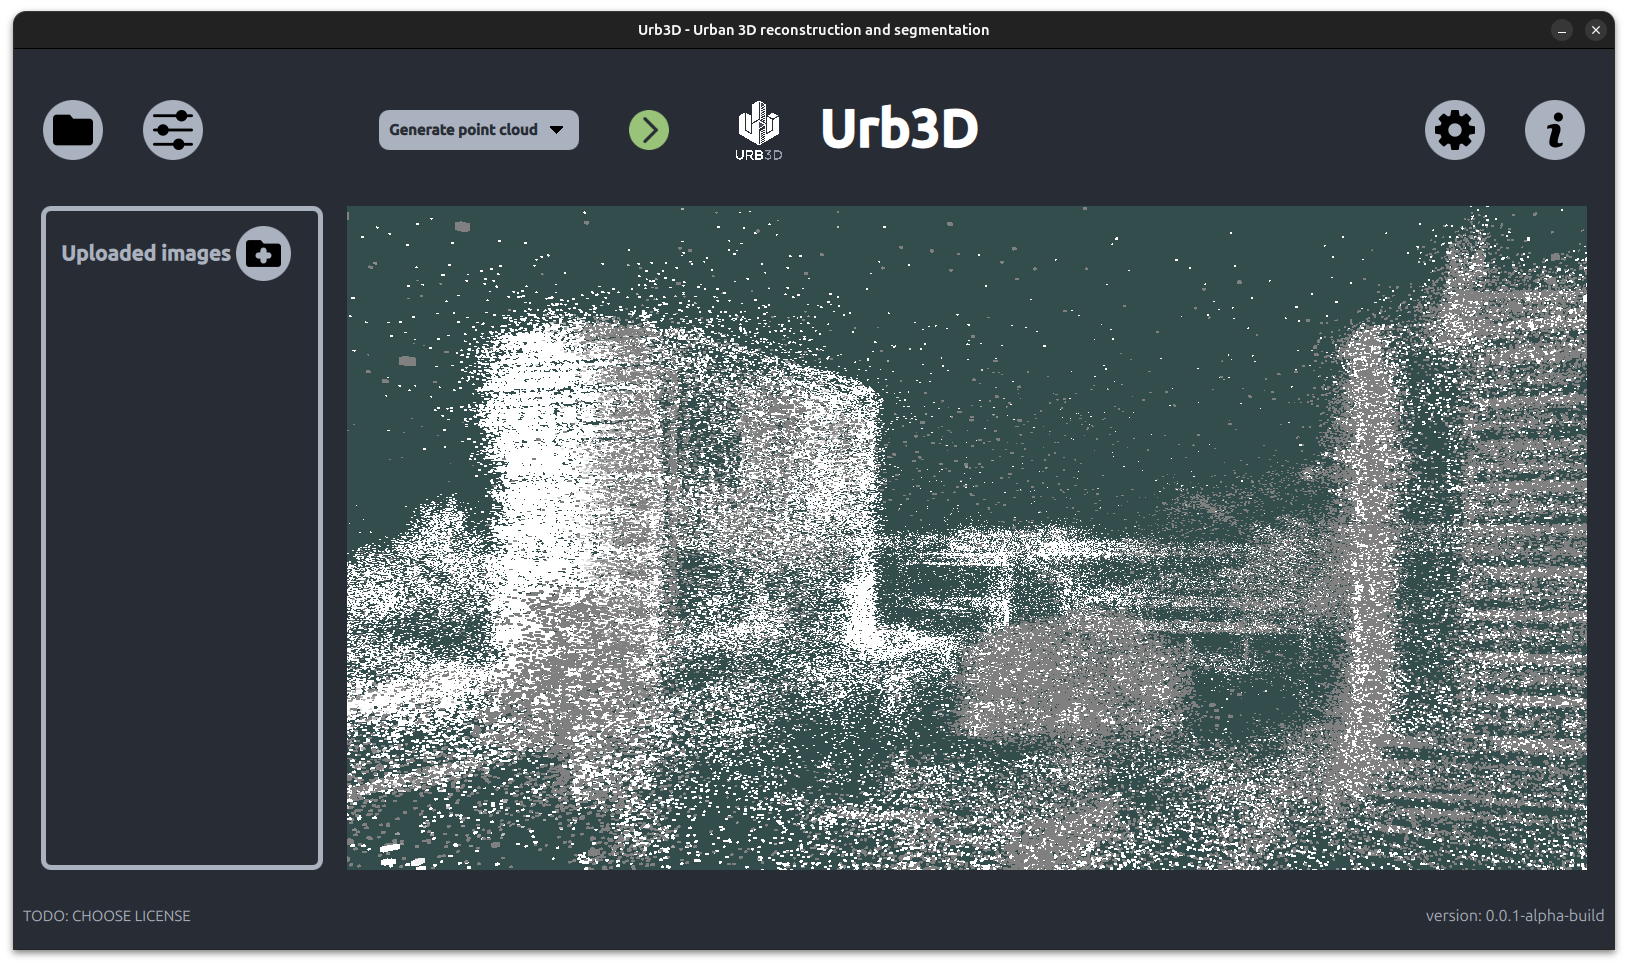
\includegraphics[width=\textwidth]{images/cloud_rendering.png}
    \caption{Zrzut ekranu przedstawiający główny widok aplikacji, w tym własny renderer}
    \label{fig:rendering}
\end{figure}